\chapter{クエリの関連文書を用いたクエリ尤度モデルの拡張}

\section{Web文書を用いたクエリ尤度モデルの拡張} \label{sec_expanddirichlet}

本研究ではディリクレスムージングのための文書コレクションとして,検索対象の文書群を用いる.
しかしクエリに関連のある文書群を検索に用いることで,クエリに対する言語モデルの表現力が向上し,より検索精度を向上させることができることが先行研究より分かっている.

% TODO: 参考文献
長谷川ら[??]は,NTCIR10のSpokenQuery\&Docタスクにおいて,web文書を用いたクエリの拡張を提案し,検索精度の改善を行っている.

そこで本研究ではWeb文書を用いたディリクレスムージングの拡張を行う.
本手法では固定文書コレクション$\theta_C$と動的文書コレクション$\theta_W$の2つを用意し,それぞれを用いて文書モデルを作成し,スムージングに用いる.
ここでは固定文書コレクションに検索対象の文書群を,動的文書コレクションに\ref{sec_webquery}節で述べる手法で収集されたWeb文書群を用いる.
式(\ref{eq_expanddirichlet})に本手法によってスムージングが行われたクエリ尤度モデルの式を示す.
\begin{flalign}
    & P(w_i|\theta_C; \mu; \nu) = \nonumber \\ 
    & \frac{|D|}{|D|+\mu+\nu}\frac{c(w_i, D)}{|D|} + \frac{\mu}{|D|+\mu+\nu}P(w_i|\theta_C) & \nonumber \\
    & + \frac{\nu}{|D|+\mu+\nu}P(w_i|\theta_W) 
    \label{eq_expanddirichlet}
\end{flalign}
ここで$P(w_i|\theta_W)$はWeb文書集合$W$内での語の生起確率であり,$\nu$はディリクレスムージングのパラメータであり,正の値を取る.

\subsection{Web 文書の取得} \label{sec_webquery}
Web文書の取得方法は,まず各クエリの単語に対してTF-IDF値を計算し,TF-IDF値のスコアの上位5単語を抽出する.そして,5単語から3単語を取り出す全て組み合わせおいて,Web検索を行い,各検索に対し10件のWeb文書を取得する.そのため,1クエリに対し,Web文書を100件取得した.最後に得られたWeb文書全てを,1つの巨大な文書とみなし,$P(w_i│θ_W)$ を計算し,式(\ref{eq_expanddirichlet})で利用する.
ここでIDFの計算に文書コレクションを利用した.

% \section{評価実験}
% \subsection{実験条件}
% 提案手法の有用性を示すため,評価実験を行なった.Web文書をクエリ尤度モデルのスムージングに利用した式(8.1)を用いた場合(スムージングパラメータ: $\alpha$ = 0.5, $\mu$ = 0.3, $\nu$ = 0.2)とWeb文書を利用せず,スムージングに文書コレクションのみを利用した場合(スムージングパラメータ: $\alpha$ = 0.5, $\mu$ = 0.5, $\nu$ = 0.0)のMAP値を比較し,本手法の有用性を調べた.また,クエリの長さに応じたMAP値の変化も調査した.ここでクエリの長さは,クエリ内に存在する名詞の個数とする.クエリの長さに応じて4分割した際の各集合の条件を表7.1に纏める.

% \begin{table}
%     \centering
%     \caption{クエリを分割したときに各集合}
%     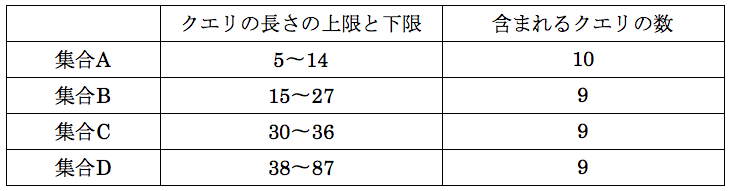
\includegraphics[width=7cm]{./image/query_set.png}
%     \label{query_set}
% \end{table}

% \subsection{実験結果}
% 実験結果を図7.1に示す.

% \begin{figure}
%     \centering
%     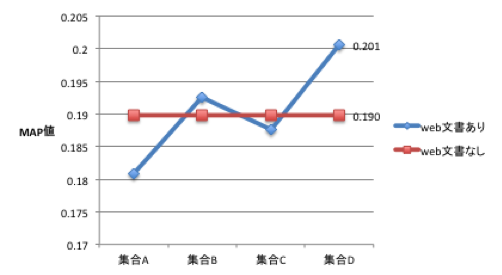
\includegraphics[width=7cm]{./image/web_result.png}
%     \caption{Web文書を利用したときのMAP値}
%     \label{web_result1}
% \end{figure}

% 図7.1よりWeb文書を用いた本手法のMAP値の最大値は,Web文書を利用していない場合より高くなった.またクエリが長いほど本手法のMAP値は上昇した.これは,クエリが長いほど,文書コレクションだけではスムージングが対応できなくなり,Web文書によるスムージングが必要になるからだと考えられる.

\section{論文を用いたクエリ尤度モデルの拡張}
Web文書と同様に論文によるクエリの情報量の拡張を図る.NTCIR11のSpokenQuery\&Docのタスクでは.検索対象文書に音響に関するプレゼンテーションの音声認識結果を提供している.クエリ尤度モデルで,\ref{sec_dirichlet}で述べたように,検索対象文書に未知語が存在する時,零確率問題を防ぐため文書コレクションを用いたスムージングによって補完するのが望ましい.そのため,文書コレクションに単語が存在しない場合に,新たな文書コレクションでスムージングする事で,よりスムージングの効果を得る事ができる.本研究では,音響の専門単語の多い,音響に関する論文を利用する事で,更なるスムージングを行う. 

\begin{flalign}
    & P(w_i|\theta_C; \mu; \nu) = \nonumber \\ 
    & \frac{|D|}{|D|+\mu+\nu}\frac{c(w_i, D)}{|D|} + \frac{\mu}{|D|+\mu+\nu}P(w_i|\theta_C) & \nonumber \\
    & + \frac{\nu}{|D|+\mu+\nu}P(w_i|\theta_P)
    \label{eq_expanddirichlet_paper}
\end{flalign}

ここで $P(w_i│θ_P)$は論文の文書集合の語 $w_i$ の生起確率である.

\subsection{論文の取得}
日本音響学会の論文について,2005年から2014年までの英語の論文を除いた8275件を用いた.
そして,各クエリとすべての論文に対し,\ref{sec_tfidf}節で述べたように,文書に対しTFを計算し,cos類似度を測ることによって,書くクエリに対し,全8275件の論文から類似度の高い論文1000件を抽出する.最後に得られたWeb文書全てを,1つの巨大な文書とみなし,$P(w_i│θ_P)$ を計算し,式(\ref{eq_expanddirichlet_paper})で利用する.

\section{評価実験}
クエリに対するクエリ尤度モデルの拡張として,Web文書と論文を利用したときの検索精度の変化を調べる.

\subsection{実験条件}

\begin{table}[htbp]
    \begin{center}
        \caption{SpokenQuery\&Doc Formal-runのSQSCR SGS retrieval条件}
        \begin{tabular}{|c|c|}
            \hline
            音声認識 & Kaldiを用いた音声認識結果 \\ \hline
            全体文書数 & 98文書 \\ \hline
            部分文書数 & 2807文書 \\ \hline
            クエリ数 & 35個 \\ \hline
        \end{tabular}
        \label{t_condition1}
    \end{center}
\end{table}

\begin{table}[htbp]
    \begin{center}
        \caption{実験条件}
        \begin{tabular}{|c|c|}
            \hline
            検索エンジン & google \\ \hline
            パラメータ $\mu$ & 320 \\ \hline
            パラメータ $\nu$ & 70 \\ \hline
        \end{tabular}
        \label{t_condition2}
    \end{center}
\end{table}

実験は,NTCIR11 SpokenQuery\&Doc Formal-run の SQSCR SGS retrieval条件で行った.
実験条件を表\ref{t_condition1}と表\ref{t_condition2}に示す.
また,特に指定しない限り,以下の実験ではクエリ・文書共に音声認識結果を用いる事とする.
Web文書は,googleの検索結果をもとに取得し,スムージングパラメータ $\mu$ と $\nu$ は経験的に定めた.
評価尺度は,\ref{sec_map}節で述べた,MAP値を用いた.

\subsection{実験結果}
実験を行った結果を表\ref{t_condition3}に示す.

\begin{table}[htbp]
    \centering
    \caption{Web文書と論文を用いたときのMAP値}
    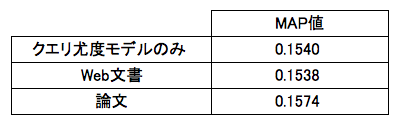
\includegraphics[width=7cm]{./image/t_condition.png}
    \label{t_condition3}
\end{table}

表\ref{t_condition3}から.論文を用いたときに,MAP値の向上が見られた.しかし,Web文書を用いたときは,MAP値にあまり変化が見られなかった.これは,Web文書がNTCIR11のクエリに対して,スムージングを行なえなかったためであると推察できる.論文を用いると,専門単語も広く言語モデルとして含められるため,スムージングできる可能性が高くなり,MAP値が上昇したのだと考えられる.

% TODO: 未知語対応がどうなのか、証拠が欲しいところ







